\chapter{Lecture}\label{part2:lec13} %% 13
\markboth{\thechapter. Lecture}{\thechapter. Lecture}

We\pageoriginale arrived at the following  result last time:
$$
\eta \left(- \frac{1}{\tau}\right) = \sqrt{\frac{\tau}{i}} \eta (\tau).
$$

We began by investigating a transformation of $\mathscr{V}_1
(\mathscr{V}, \tau)$. Instead of looking upon 1 and $\tau$ as
generators of the period lattice, we looked upon $\tau$ and $-1$ as
generators (turning the plane around through arg $\tau$): 1, $\tau \to
\tau, -1$. We have of course still the same parallelogram of
periods. Since we should like to keep the first period 1, we reduced
everything by $\tau: \tau, -1 \to 1, - \frac{1}{\tau}$; so we had to
investigate $\mathscr{V}_1 (\mathscr{V} \tau/\tau)$. $\mathscr{V}_1 (
\mathscr{V} \tau/\tau)$ and $\mathscr{V}_1
(\mathscr{V}/-\frac{1}{\tau})$ have the same parallelogram of
periods. 

We could do this a little more generally. Let us introduce linear
combinations: 
$$
\omega_1 = c \tau+d, \quad \omega_2=a\tau +b,
$$

\noindent 
\begin{minipage}[c]{4.5cm}
  and go from $\omega_1$ to $\omega_2$ in the positive sense. In order
  that we must have these also as generating vectors for the same
  lattice, we should have $a$, $b$, $c$, $d$ integers with
  $$
  \begin{vmatrix}
    a & b\\
    c & d
  \end{vmatrix}= 1.
  $$
\end{minipage}
\begin{minipage}[c]{5cm}
  \begin{figure}[H]
    \centering{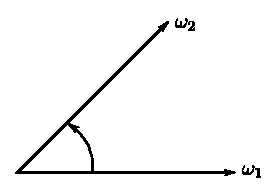
\includegraphics{vol2-figures/fig2.18.eps}}
  \end{figure}
\end{minipage}

Moreover we want the first period to be always 1. (This is the
difference between our case and the Weierstrassian introduction of
periods, where we have complete homogeneity). So replacing by
linearity, the periods are 1 and $\tau'=\frac{a \tau + b}{c\tau+d}$. 

Be\pageoriginale sure that we want to go from 1 to $\tau'$ through an
angle less than $\pi$ in the positive sense. For this we want $\tau'$
to have a positive imaginary parts $Im \bar{\tau}' > 0$, or
$$
\displaylines{\hfill \frac{\tau'- \bar{\tau}'}{i} > 0 \hfill \cr
\text{i.e.,} \hfill \frac{1}{i} \left(\frac{a \tau+b}{c\bar{\tau}+d} -
\frac{a \bar{\tau}+b}{c\bar{\tau}+d}\right) > 0 \hfill \cr
\text{i.e.,} \hfill \frac{1}{i} \frac{ad \tau + bc \bar{\tau}- ad
  \bar{\tau}- bc \tau}{|c\tau + d|^2}> 0 \hfill \cr
\text{i.e.,} \hfill\frac{1}{i} \frac{(ad-bc)(\tau -
  \bar{\tau})}{|c\tau + d|^2} > 0 \hfill }
$$
or since $\tau - \bar{\tau}$ is purely imaginary,
$$
ad - bc = \pm 1.
$$

We could do the same thing in all our different steps. The most
important step, however, cannot be carried through, because we get
lost at an important point; and rightly so, it becomes cumber some
because a number-theoretic problem is involved there. Let us see what
we have done. Compare
$$
\mathscr{V}_1 ((c\tau + d)\mathscr{V}/\tau)~\text{and}~ \mathscr{V}_1
\left(\mathscr{V}\Big/ \frac{a \tau+b}{c\tau +d}\right)
$$

We want periods 1, $\tau'$; indeed all things obtainable from
$\omega_1= c \tau + d$ and $\omega_2 = a \tau+ b$; or $m_1\omega_1+
m_2 \omega_2$ must in their totality comprise all periods. For the
first $c \tau +d$ is indeed a period, and for the second $a \tau+b$. 

Now\pageoriginale define
$$
f(\mathscr{V}) = \mathscr{V}_1 ((c\tau+ d)\mathscr{V}/\tau)
$$
$f(\mathscr{V}+1)$ is essentially $f(\mathscr{V})$:
\begin{align*}
  f(\mathscr{V}+1) & = \mathscr{V}_1 ((c \tau +d)\mathscr{V}+ c\tau
  +d/\tau)\\
  & = (-)^{c+d} e^{- {c^2} \pi i \tau} e^{- ***** (c \tau
    +d)\mathscr{V}} \mathscr{V}_1((c \tau +d)\mathscr{V}/\tau),
  ~\text{from the table},\\
  & = (\cdots\cdots) f (\mathscr{V})\\
  f(\mathscr{V}+ \tau') & = \mathscr{V}_1 ((c \tau +d) \nu + a \tau +
  b/ \tau)\\
  & = (-)^{a+b} e^{- {a^2}\pi i \tau} e^{-2\pi i a(c \tau + d)\nu}
  \mathscr{V}_1 ((c \tau +d)\mathscr{V}/\tau)\\
  & = (\cdots\cdots) f(\mathscr{V})
\end{align*}

$f(\mathscr{V})$ has, leaving trivial factors aside, periods 1,
$\tau'$ *****. So too for the second function $\mathscr{V}_1
\left(\mathscr{V}\Big/ \frac{a \tau+ b}{c\tau + d}\right)$.

We can form quotients and proceed as we did earlier. 

Let us consider for a moment the $\mathscr{V}'s$ with double
subscripts. This is a digression, but teaches us a good deal about how
to work with $\mathscr{V}$-functions. Recall that 
\begin{align*}
  \mathscr{V}_{\mu \nu}(\nu/\tau) &= \sum_{n} (-)^{\nu n} e^{\pi i
    \tau \left(n + \frac{1}{2}\right)^2} e^{2 \pi i \nu \left(n+
    \frac{1}{2}\right)}\\
  \mathscr{V}_1 (\nu/ \tau) & = \mathscr{V}_n (\nu/\tau)\\
  \mathscr{V}_2 (\nu/\tau) & = \mathscr{V}_{10} (\nu/\tau)\\
  \mathscr{V}_3(\nu/\tau) & = \mathscr{V}_{00} (\nu\tau)\\
  \mathscr{V}_4 (\nu /\tau) & = \mathscr{V}_{01} (\nu/\tau)
\end{align*}

We\pageoriginale take one liberty from now on. Take $\mu, \nu$ to be
arbitrary integers, no longer 0, 1. That will not do very much harm
either. In fact,
$$
\mathscr{V}_{\mu , \nu+2} (\nu/\tau)= \mathscr{V}_{\mu, \nu} (v/\tau)
$$

It is unfortunately not quite so easy for the other one:
$$
\mathscr{V}_{\mu +2, \nu} (v/\tau)= (-)^\nu \mathscr{V}_{\mu,\nu} (v/\tau)
$$

For 
\begin{align*}
  \mathscr{V}_{\mu +2, \nu} (v/\tau) & = \sum_{n} (-)^{\nu} e^{\pi i
    \tau(n +\mu /2)^2} e^{2 \pi i \nu (n+1+\mu/2)}\\
  & = \sum_{n} (-)^{\nu} (-)^{v(n+1)} e^{\pi i \tau (n+1+ \mu/2)^2} e^{2
    \pi i v (n+1+\mu/2)}\\
  & = (-)^v \mathscr{V}_{\mu \nu} (v/\tau),
\end{align*}
on shifting the summation index from $n$ to $n+ 1$. The original table
will be considerably reduced now; only in place of $\nu+1$, $\nu+
\frac{1}{2}$, $\nu+ \frac{\tau}{2}$, $\nu+ \frac{1+\tau}{2}$ it will
be now necessary to have the combination $\nu +\frac{k}{2} +
\frac{l}{2} \tau$. The expression for $\mathscr{V}_{\mu \nu} \left(\nu
+ \dfrac{k}{2} + \dfrac{l}{2}  \tau/ \tau \right)$ will include
everything that we have done so far in one single formula. 
\begin{align*}
  \mathscr{V}_{\mu \nu} \left( \nu + \frac{k}{2} + \frac{l}{2}
  \tau/\tau\right)  & = \sum_{n} (-)^{\nu n} e^{\pi i \tau (n+
    \frac{\mu}{2})^2} e^{2 \pi i \nu (n+ \frac{\mu}{2})} e^{\pi i (k+l
    \tau)(n+ \frac{\mu}{2})}\\
  & = i^{k \mu} \sum_n (-)^{(\nu+ k)^n} e^{\pi i \tau(n+ \mu/2+
    l/2)^2} e^{- \pi i \tau l^2/4} e^{2 \pi i \nu (n+ \mu/2+l/2)} e^{-
  \pi i l \nu}\\
  & = i^{k \mu} e^{-\pi i \tau l^2/4} e^{- \pi i l \nu}
  \mathscr{V}_{\mu +l, \nu+k} (\nu/\tau) \tag{*}
\end{align*}\pageoriginale 

This one formula has the whole table in it.

We now turn to our purpose, viz. To consider the quotient
$$
\frac{\mathscr{V}_1 ((c \tau+d)\nu/\tau)}{\mathscr{V}_1 \left(\nu \Big/
  \frac{a \tau+b}{c \tau +d}\right)}
$$

We wish to discuss the behaviour a little more explicitly of $f(\nu)$.
\begin{align*}
  f(v) & = \mathscr{V}_{11} ((c \tau+d) \nu/\tau)\\
  f(v+1) & = \mathscr{V}_{11} ((c \tau +d)\nu + c\tau +d/\tau)\\
  f(v+\tau') & = \mathscr{V}_{11} ((c \tau +d)\nu + a \tau + b/ \tau)
\end{align*}
putting\pageoriginale $k=2c$, $l=2d$, $\mu=\nu=1$ in (*), 
\begin{align*}
  f(\nu+1) & = (-)^d e^{-\pi i \tau c^2} e^{-2 \pi i c(c \tau + d)\nu}
  \mathscr{V}_{1+2c, 1+2d} ((c\tau+d)\nu /\tau)\\
  & = (-)^{c+d} e^{-\pi i \tau c^2} e^{-\pi i c(c \tau +d)\nu} f(v)
\end{align*}

Similarly, putting $k = 2a$, $l= 2b$, $\mu=\nu=1$, 
$$
f(\nu + \tau') = (-)^{a+b} e^{- \pi i \tau a^2} e^{-2 \pi i a (c \tau
  + d) \nu} f(v).
$$

Also defining $g(\nu)$:
$$
\mathscr{V}_1 \left(v\Big/\frac{a \tau + b}{c \tau +d} \right) = g(v)
= \mathscr{V}_{11} (\nu/\tau'),
$$
we have
$$
g(\nu+1) = \mathscr{V}_{11} (\nu + 1/\tau')=- \mathscr{V}_{11} (\nu/ \tau').
$$

And putting $k=0$, $l=2$, $\mu=3$, $\nu=1$ in (*),
\begin{align*}
  g(\nu+ \tau') & = e^{- \pi i \tau'} e^{- 2 \pi i \nu}
    \mathscr{V}_{31} (\nu/\tau')\\
    & = - e^{- \pi i \tau'} e^{-2 \pi i \nu} g(\nu).
\end{align*}

We form now in complete analogy with the old procedure
\begin{align*}
 \Phi (\nu) & = \frac{f(\nu)}{g(\nu)}\\
 \Phi (\nu+1) & = (-)^{c+d+1} e^{- \pi i \tau c^2} e^{-2 \pi i c(c
   \tau + d)\nu \Phi (\nu)},\\
 \Phi (\nu + \tau') & = (-)^{a+b+1} e^{- \pi i \tau c^2} e^{- 2\pi i a
 (c \tau+d)\nu} e^{\pi i \tau' + 2 \pi i v} \Phi (\nu)
\end{align*}

$\Phi$\pageoriginale takes up exponential factors which contain $\nu$
linearly. As before ewe can submerge this under a general form. Define 
$$
\Psi (\nu) = \Phi (\nu) e^{h(\nu)},
$$
where $h(\nu)$ is to be so determined that
$$
\Psi (\nu+1) = \Psi (\nu + \tau') = \Psi (\nu)
$$
we therefore want
\begin{align*}
  e^{h(\nu+1)- h(\nu)} (-)^{c+d+1} e^{-c^2 \pi i \tau -2 \pi i c(c\tau
    +d)\nu}& =1,\\
  e^{h(\nu+\tau')- h(\nu)} (-)^{a+b+1} e^{-a^2 \pi i \tau + \pi i
    \tau'+ 2 \pi i \nu} e^{- 2 \pi i a (c\tau +d)\nu} & =1.  
\end{align*}

It will be convenient to observe that $c+d+cd+1= (c+1)(d+1)$ is even,
for at least one of $c$, $d$ should be odd as otherwise $c$, $d$ would
not be co-prime and we would not have 
$$
\begin{vmatrix} 
  a & b\\ 
  c & d 
\end{vmatrix} =1
$$

So $(-)^{c+d+1} = (-)^{cd} = e^{\pi i cd}$. $h$ is given by the
equations:
\begin{align*}
  h(\nu+1)- h(\nu) & = 2 \pi i c(c \tau + d) \nu + \pi i c (c \tau
  +d),\\
  h(\nu+ \tau') - h(\nu) & = 2 \pi i a (c\tau +d) + \pi i a(a \tau +b)
  - \pi i \tau'\\
  & = 2 \pi c (a \tau +b) \nu + \pi i c \tau' (a \tau +b).
\end{align*}

We have to introduce a suitable function $h(\nu)$. Since the
difference equation can be solved by means of a second degree
polynomial, put
$$
h(\nu)= A \nu^2 + B
$$
for\pageoriginale each separately and see whether it works for both.
\begin{align*}
  h(\nu+\delta) - h(\nu)& = 2 A \nu \delta  + A \delta^2 + B \delta\\
  & = \delta (2 A \nu + A \delta + B)
\end{align*}

Putting $\delta= 1$, $\tau'$, we find that $A= \pi i c (c \tau +d)$
works in both cases. Also for $\delta=1$,
\begin{gather*}
A+B = \pi i c(c\tau +d),\\
A\left( \frac{a \tau+b}{c\tau+d}\right)^2 + B \left(\frac{a \tau +b}{c
  \tau+d}\right)  = \frac{\pi i c (a \tau +b)^2}{c\tau +d}
\end{gather*}

So $B=0$ fits both. Hence
\begin{alignat*}{4}
  &\hspace{1cm}& h(\nu) & = A \nu^2, A = \pi i (c \tau +d) c\\
  \therefore && \Psi (\nu) & = e^{\pi i c (c \tau +d) \nu^2} \frac{f(\nu)}{g(\nu)}
\end{alignat*}

And this is a doubly periodic entire function (because the numerator
and denominator have the same simple zeros) and therefore a
constant. We thus have the transformation formula
$$
\mathscr{V}_{11} \left(\nu \Big/ \frac{a \tau+b}{c\tau+d}\right) =
C e^{\pi i c (c \tau +d)\nu^2} \mathscr{V}_{11}((c \tau+d)\nu/\tau)
$$
where $C$ may depend on the parameters $\tau, a, b, c, d$:
$$
C= C(\tau; a, b, c, d)
$$

More\pageoriginale generally we can have a parallel formula for any
$\mu, \nu$. As before we get an equation for $C^2$. And there the
thing stops. Formerly we were in a very good position with the special
matrix
$$
\begin{pmatrix}
a & b\\
c & d
\end{pmatrix}= 
\begin{pmatrix}
  0 & -1\\
  1 & 0
\end{pmatrix}.
$$

For general $a$, $b$, $c$, $d$ we get into trouble. 


